\chapter{Patrones}
\section{Patrones}

\subsection{Creacionales}

\bigskip

\subsubsection{Builder}

\begin{figure}[th!]
	\centering
	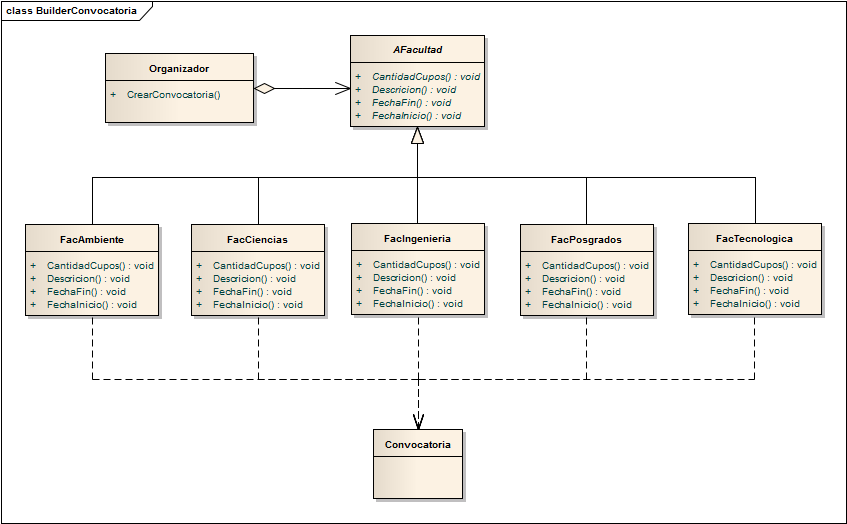
\includegraphics[width=1.2\linewidth]{uml/Patrones/BuilderConvocatoria}
	\caption{Builder para crear convocatoria}
	\label{fig:Builder para convocatoria}
\end{figure}

\clearpage

\subsubsection{Factory}
\begin{figure}[th!]
	\centering
	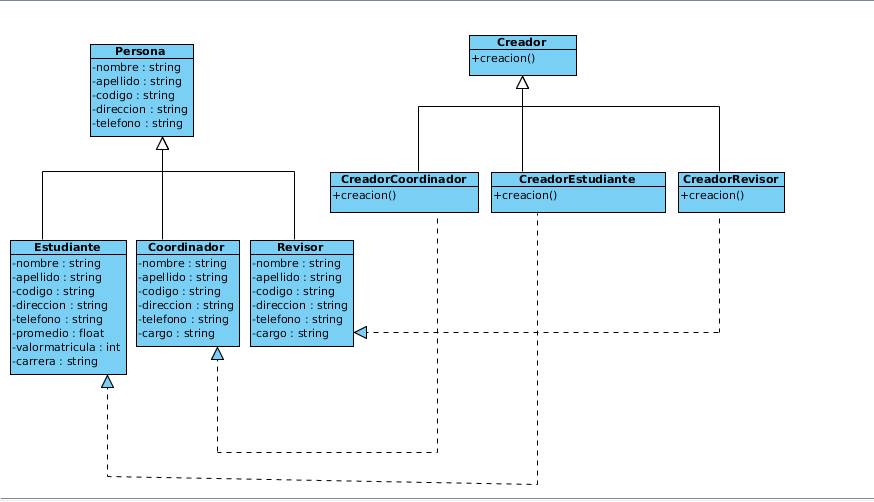
\includegraphics[width=1.2\linewidth]{uml/Patrones/FactoryMethod}
	\caption{Fabrica para crear personas}
	\label{fig:Fabrica para crear personas}
\end{figure}

\clearpage

\subsubsection{Singleton}
\begin{figure}[th!]
	\centering
	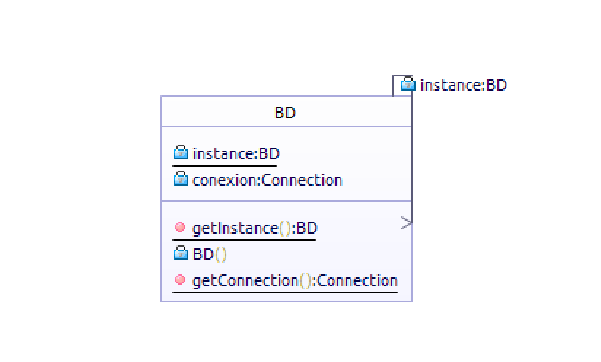
\includegraphics[width=1.2\linewidth]{uml/Patrones/Singleton}
	\caption{Singleton para conexion con la base de datos}
	\label{fig:Singleton}
\end{figure}

\clearpage



\newpage

\subsection{Estructurales}

\newpage

\subsection{Comportamiento}

\subsubsection{Iterador}
\begin{figure}[th!]
	\centering
	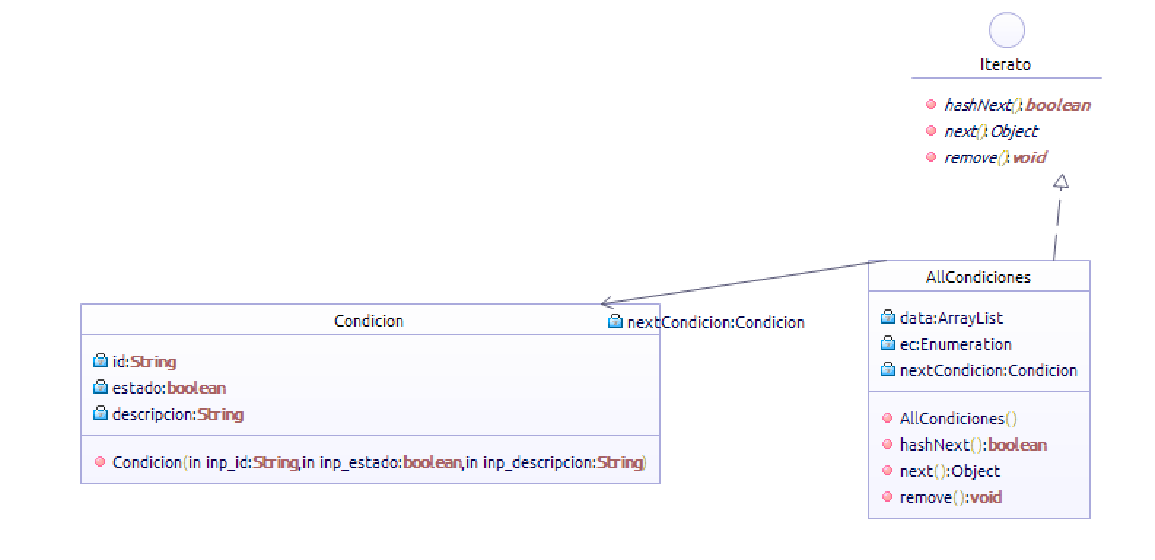
\includegraphics[width=1.2\linewidth]{uml/Patrones/Iterador}
	\caption{Iterador, muestra listado de condiciones para el apoyo}
	\label{fig:Iterador}
\end{figure}
\newpage
\subsubsection{State}
\begin{figure}[th!]
	\centering
	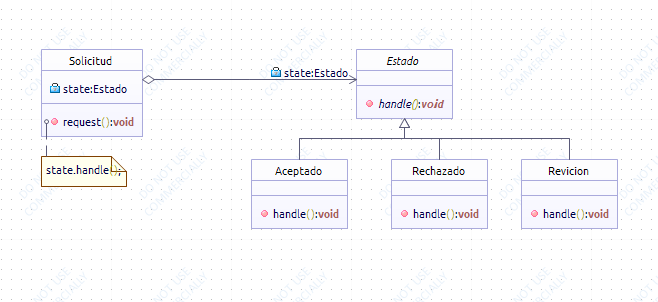
\includegraphics[width=1.2\linewidth]{uml/Patrones/Estado}
	\caption{Estado, Muestra los estados de las solicitudes}
	\label{fig:Estado}
\end{figure}

\clearpage



%\section{Diagrama de Objetos}

%\newpage

%\section{Diagrama de Estructura Compuesta}

%\newpage